\section{Мета}
Вивчення механізму переривань, їх типів, алгоритму та
засобів їхньої обробки, а також набуття практичних навичок створення
власних програм обробки переривань.

\section{Завдання}
озробити власну процедуру обробки переривання (див. 3.5.1.4),
яка б виконувала такі дії:
\begin{enumerate}
    \item виклик програми обробки переривання (див. п. 3.5.1.3) з одним із номерів переривання, зарезервованих для користувача (див. табл. 3.1 );
    \item аналіз стану заданої клавіші-перемикача згідно з таблицею 3.2;
    \item при натисканні кнопки – виведення на екран її назви
\end{enumerate}

\section{Хід роботи}
\subsection{Код програми}
\lstinputlisting[language=Rust, style=colouredRust]{\codeDirectory/lab3/main.c}

\subsection{Результат роботи програми}
\begin{figure}[ht!]
    \centering
    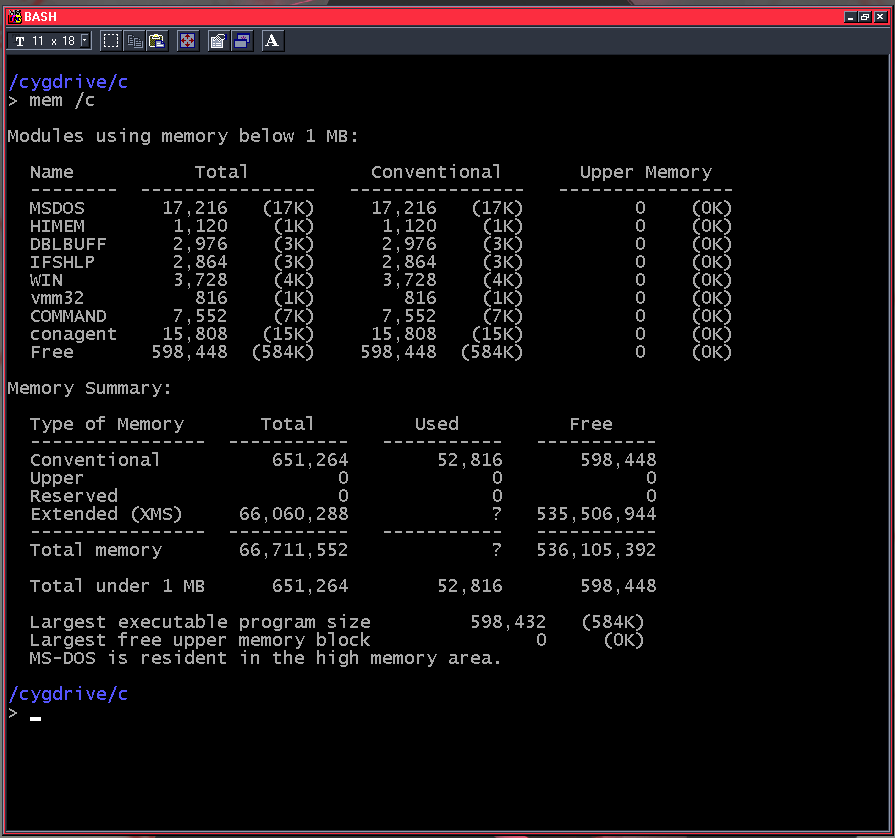
\includegraphics[width=0.9\textwidth]{\assetsDirectory/lab3_1.png}
    \caption{Запушені процеси до запуску програми}
\end{figure}
\begin{figure}[ht!]
    \centering
    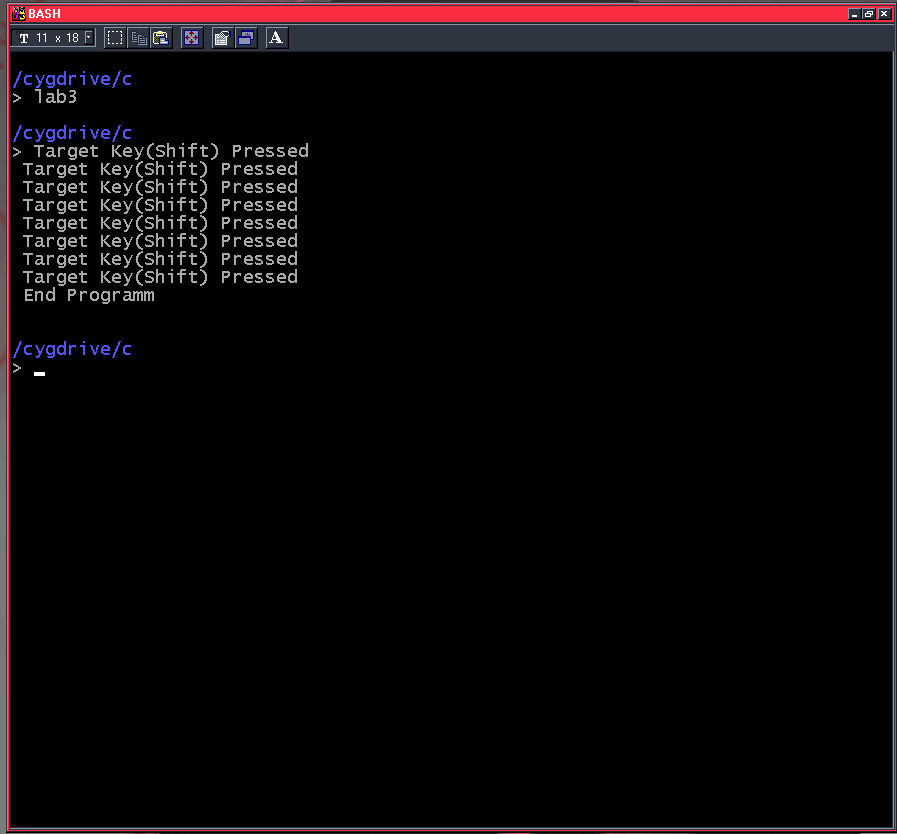
\includegraphics[width=0.9\textwidth]{\assetsDirectory/lab3_2.png}
    \caption{Приклад роботи програми}
\end{figure}
\begin{figure}[ht!]
    \centering
    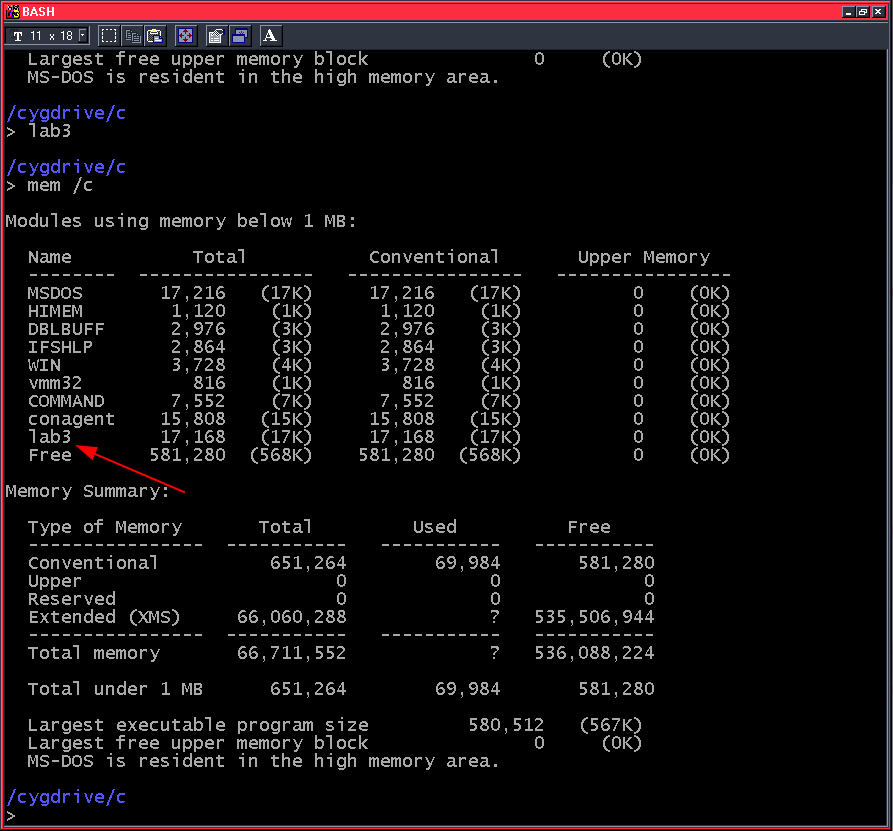
\includegraphics[width=0.9\textwidth]{\assetsDirectory/lab3_3.png}
    \caption{Запушені процеси після запуску програми}
\end{figure}

\clearpage
\section{Висновки}
У ході виконання лабораторної роботи було здобуто практичні навички створення користувацьких переривань.
Також розроблено програму, яка обробляє натискання клавіші RightShift за допомогою власної процедури обробки переривань.
